%%%%%%%%%%%%%%%%%%%%%%%%%%%%%%%%%%%%%%%%%%%%%%%%%%%%%%%%%%%%%%%%%%%%%%
% Slides
%%%%%%%%%%%%%%%%%%%%%%%%%%%%%%%%%%%%%%%%%%%%%%%%%%%%%%%%%%%%%%%%%%%%%%

\begin{frame}
\titlepage
\end{frame}

\begin{frame}{Roteiro}
  \tableofcontents
\end{frame}

\section{Introdução}

\begin{frame}{Cassandra}
\begin{itemize}

\item Distribuido e Descentralizado
\item Elasticamente Escalável
\item Altamente Disponível e Tolerante a Falhas
\item Variavelmente Consistente

\end{itemize}
\end{frame}

\begin{frame}{Bolsa Família}
  \begin{itemize}
    \item Programa de transferência de renda para famílias em pobreza ou extrema pobreza
    \item 13,9 milhões de família com um custo anual de R\$27,4 bilhões 
  \end{itemize}
\end{frame}

\section{Estudo de Caso}
\begin{frame}{Estudo de Caso}
  \begin{itemize}
    \item Portal da Transparência
    \item 24 arquivos no total
    \item 16Gib e quase 14 milhões de registros por arquivo
\end{itemize}

Campos: \textbf{UF, Código SIAFI Município, Nome Município, Código Função, Código Subfunção, Código Programa, Código Ação, NIS Favorecido, Nome Favorecido, Fonte-Finalidade, Valor Parcela e Mês Competência}

\end{frame}

\begin{frame}{Modelo de Dados}
	\begin{itemize}
		\item Fator de replicação 1(sem tolerância a falhas)
		\item UF, Código SIAFI Município, Nome Município, NIS Favorecido, Nome Favorecido, Fonte-Finalidade,
		Valor Parcela, Mês Competência
		\item Chave primária: \textbf{UF}, NIS Favorecido,
		Valor Parcela e Mês Competência
	\end{itemize}
	
\end{frame}

\begin{frame}{Aplicação}
	Foi desenvolvida uma aplicação em Java, com uso do driver da Datastax.
	A aplicação realiza ETL dos arquivos .csv originais, e consultas no banco por meio de CQL.
\end{frame}

\begin{frame}{Testes}
	Inserção e Busca realizadas por meio de comandos CQL na aplicação, com uso do driver da Datastax
	\begin{itemize}
		\item 2, 4, 6 máquinas
		\item 6 meses, 1 ano, 2 anos
	\end{itemize}
\end{frame}

\section{Resultados}

\begin{frame}{Resultados Obtidos}

\begin{figure}[!htb]
	\centering
	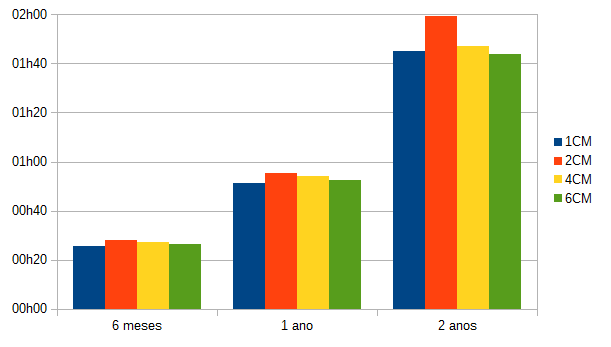
\includegraphics[width=1\textwidth]{../figuras/graphinsert.png}
	\caption{Inserção de dados}
	\label{fig:graphinsert}
\end{figure}
  
\end{frame}

